\documentclass{article}


\usepackage{arxiv}

\usepackage[utf8]{inputenc} % allow utf-8 input
\usepackage[T1]{fontenc}    % use 8-bit T1 fonts
\usepackage{hyperref}       % hyperlinks
\usepackage{url}            % simple URL typesetting
\usepackage{booktabs}       % professional-quality tables
\usepackage{amsfonts}       % blackboard math symbols
\usepackage{nicefrac}       % compact symbols for 1/2, etc.
\usepackage{microtype}      % microtypography
\usepackage{lipsum}
\usepackage{graphicx}
\usepackage{subcaption}
\graphicspath{ {./images/} }


\title{Deep Graph Library - raport techniczny}


\author{
 Zawalska Justyna \\
  Wydział Informatyki, Elektroniki i Telekomunikacji\\
  Akademia Górniczo-Hutnicza \\
  Kraków \\
  \texttt{jzawalska@student.agh.edu.pl} \\
  \And
 Gędłek Paweł \\
  Wydział Informatyki, Elektroniki i Telekomunikacji\\
  Akademia Górniczo-Hutnicza \\
  Kraków \\
  \texttt{gedlek@student.agh.edu.pl} \\
  \And
 Pęczek Paweł \\
  Wydział Informatyki, Elektroniki i Telekomunikacji\\
  Akademia Górniczo-Hutnicza \\
  Kraków \\
  \texttt{peczek@student.agh.edu.pl} \\
}


\begin{document}
\maketitle
\begin{abstract}
Przetwarzanie grafów stanowi obecnie istotną cześć całości przetwarzania danych. Ma to związek z elasycznością grafu jako modelu przedstawiania wiedzy. W związku z rosnącym zapotrzebowaniem na narzędzia do wydajnego i skutecznego pozyskiwania informacji ze struktur grafowych widoczna jest tendencja do poszukiwania nowych metod udoskonalających obecny stan wiedzy z tego zakresu. Jednym z nowatorskich sposobów przetwarzania grafów jest wykorzystanie sieci neuronowych. Jako skutek upowszechnienia tej idei powstawają biblioteki pozwalające na zastosowanie osiągnięć z tej dziedziny do rozwiąznia praktycznych problemów na szeroką skalę. W ramach tego dokumentu przedstawiamy owoce eksploracji biblioteki Deep Graph Library (DGL) plasującej się w wyżej wymienionej kategorii. Naszym wkładem jest zbadanie jej możliwości i ograniczeń poprzez wykonanie serii eksperymentów będących próbą zastosowania DGL do rozwiązania praktycznych problemów z zakresu przetwarzania grafów.
\end{abstract}


% keywords can be removed
%\keywords{First keyword \and Second keyword \and More}


\section{Struktura raportu}
\label{sec:report_structure}
\paragraph{}
Organizacja niniejszego dokumentu jest następująca. Sekcja \ref{sec:intro} zawiera opis istoty działania biblioteki DGL \cite{dgl}. W sekcji \ref{sec:dgl_structure} znajduje się opis istotnych elementów struktury biblioteki i jej ocena. Sekcja \ref{sec:dgl_system_requirements} prezentuje wymagania techniczne. W dalszej kolejności, sekcja \ref{sec:experiments} zawiera podsumowanie eksperymentów, które zostały przeprowadzone z wykorzystaniem biblioteki DGL \cite{dgl}, ze szczególnym uwzględnieniem aspektów związanych z użytecznością różnych sposobów reprezentacji grafów oraz analizą jakości rozwiązań zaproponowanych przez twórców DGL \cite{dgl}. Całość raportu dopełniają wnioski wyciągnięte z przeprowadzonych badań, które są zaprezentowane w sekcji \ref{sec:conclusions}.

\section{Wstęp}
\label{sec:intro}
W naszym projekcie użyliśmy biblioteki DGL w wersji 0.43, można więc założyć, że w pewnym stopniu niektóre jej elementy są jeszcze w fazie eksperymentalnej. Świadczy o tym chociażby fakt, że w tej wersji API próbkowania w  heterografach zostało wprowadzone jako experimental, a także dopiero od tej wersji został dodany pełny support dla biblioteki Tensorflow.
\paragraph{}
Twórcy bibliotei DGL postanowili poddać ją testom wydajnościowym oraz skalowania. Używając funkcji tensorowych z backendowych frameworków takich jak PyTorch, MXNet, czy Tensorflow DGL w bardzo dużym stopniu optymalizuję zużycia pamięciowe i obliczeniowe, dzięki swoim własnym kernelom. Poniżej prezentujemy porównanie do innego podobnego pakietu PyTorch Geometric (PyG). W tabeli zostały umieszczone czasy w sekundach dla 200 epok oraz zużycie pamięci w GB.

\begin{table}
\begin{center}
\begin{tabular}{ |c|c|c|c|c|c|c|c| } 
Dataset  & Model                                             & Acurracy                      & \multicolumn{2}{c}{Time} & \multicolumn{2}{c}{Memory} \\
         &                                                   &                               & PyG         & DGL        & PyG          & DGL         \\
\hline
Cora     & \begin{tabular}[c]{@{}l@{}}GCN\\ GAT\end{tabular} & \begin{tabular}[c]{@{}l@{}}$81.31 \pm 0.88$ \\ $83.98 \pm 0.52$\end{tabular} &       \begin{tabular}[c]{@{}l@{}} 0.478 \\ 1.608 \end{tabular}        &       \begin{tabular}[c]{@{}l@{}} 0.666 \\ 1.399 \end{tabular}       &       \begin{tabular}[c]{@{}l@{}} 1.1 \\ 1.2 \end{tabular}      &      \begin{tabular}[c]{@{}l@{}} 1.1 \\ 1.1 \end{tabular}           \\
\hline
CiteSeer & \begin{tabular}[c]{@{}l@{}}GCN\\ GAT\end{tabular} & \begin{tabular}[c]{@{}l@{}}$70.98 \pm 0.68$ \\ $69.96 \pm 0.53$\end{tabular} &        \begin{tabular}[c]{@{}l@{}} 0.490 \\ 0.674 \end{tabular}        &      \begin{tabular}[c]{@{}l@{}} 0.674 \\ 1.399 \end{tabular}       &       \begin{tabular}[c]{@{}l@{}} 1.1 \\ 1.3 \end{tabular}      &      \begin{tabular}[c]{@{}l@{}} 1.1 \\ 1.1 \end{tabular}           \\
\hline
PubMed   & \begin{tabular}[c]{@{}l@{}}GCN\\ GAT\end{tabular} & \begin{tabular}[c]{@{}l@{}}$79.00 \pm 0.41$ \\ $77.65 \pm 0.32$\end{tabular} &         \begin{tabular}[c]{@{}l@{}} 0.491 \\ 1.946 \end{tabular}       &      \begin{tabular}[c]{@{}l@{}} 0.690 \\ 1.393 \end{tabular}       &       \begin{tabular}[c]{@{}l@{}} 1.1 \\ 1.6 \end{tabular}      &      \begin{tabular}[c]{@{}l@{}} 1.1 \\ 1.1 \end{tabular}           \\
\hline
Reddit   & GCN                                               & $ 93.46 \pm 0.06$ &      OOM         &    28.6         &      OOM      &      11.7         \\
\hline
Reddit-S & GCN                                               & N/A &        29.12       &      9.44        &      15.7       &     3.6             
\end{tabular}
\end{center}
\end{table}

\begin{figure}
\centering
\begin{subfigure}{.5\textwidth}
  \centering
  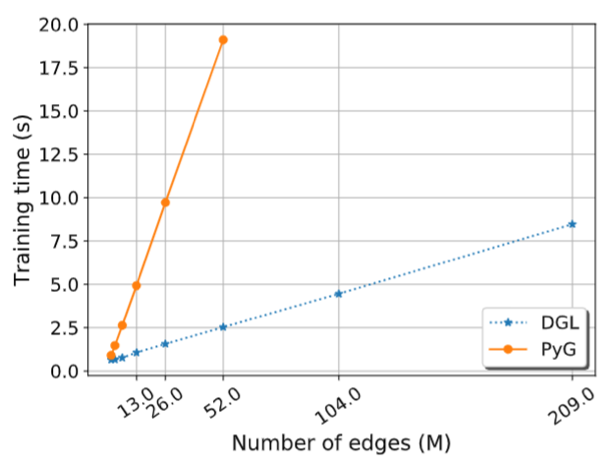
\includegraphics[width=0.9\linewidth]{images/DGLvsPyG-time1}
  \label{fig:sub1}
\end{subfigure}%
\begin{subfigure}{.5\textwidth}
  \centering
  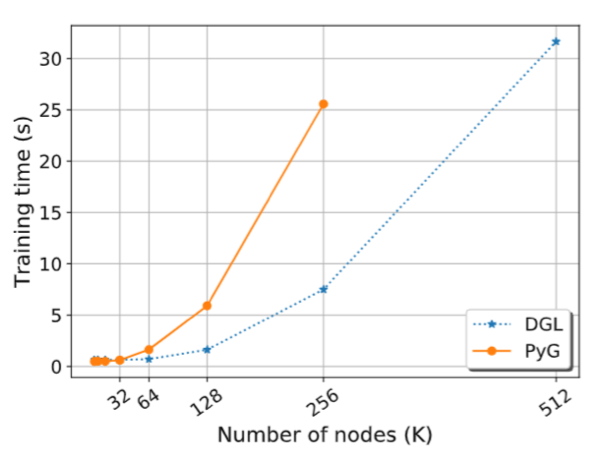
\includegraphics[width=0.9\linewidth]{images/DGLvsPyG-time2}
  \label{fig:sub2}
\end{subfigure}
\caption{Porównanie czasów dla obu bibliotek}
\label{fig:test}
\end{figure}

W kwestii skalowalności biblioteka DGL wygląda naprawdę dobrze na tle konkurencji. W dużym stopniu wykorzystuję możliwości obliczeń na wielu GPU zarówno na jednej maszynie jak i na klastrach obliczeniowych, w celu przyspieszenia szybkości treningu. 

\begin{figure}[h]
\centering
\begin{subfigure}{.5\textwidth}
  \centering
  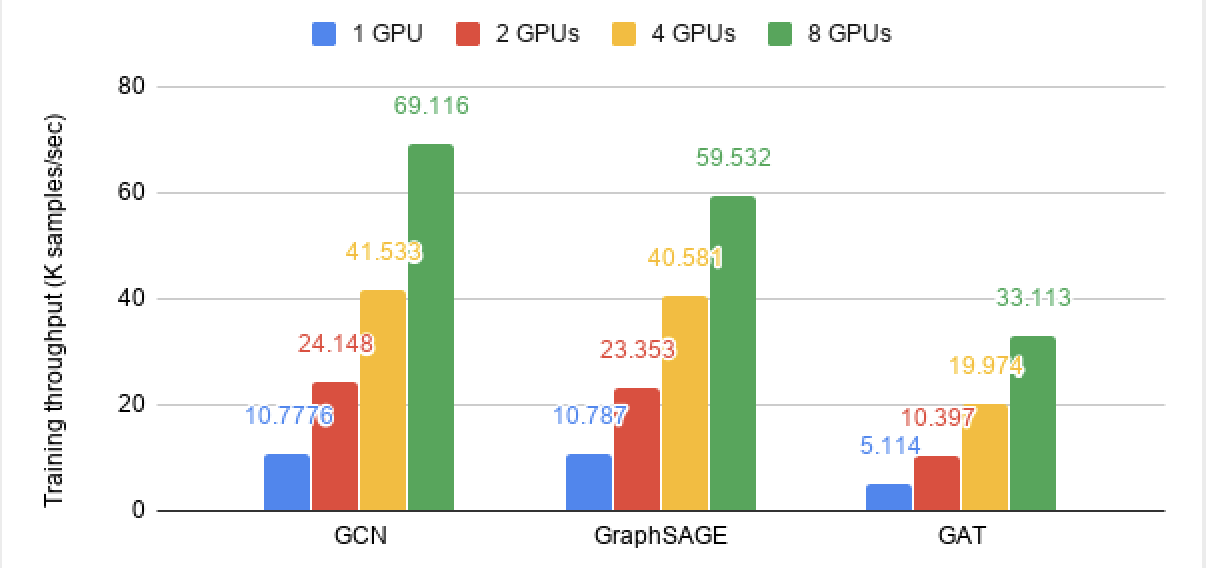
\includegraphics[width=0.9\linewidth]{images/one-four-GPUs}
  \label{fig:sub1}
\end{subfigure}%
\begin{subfigure}{.5\textwidth}
  \centering
  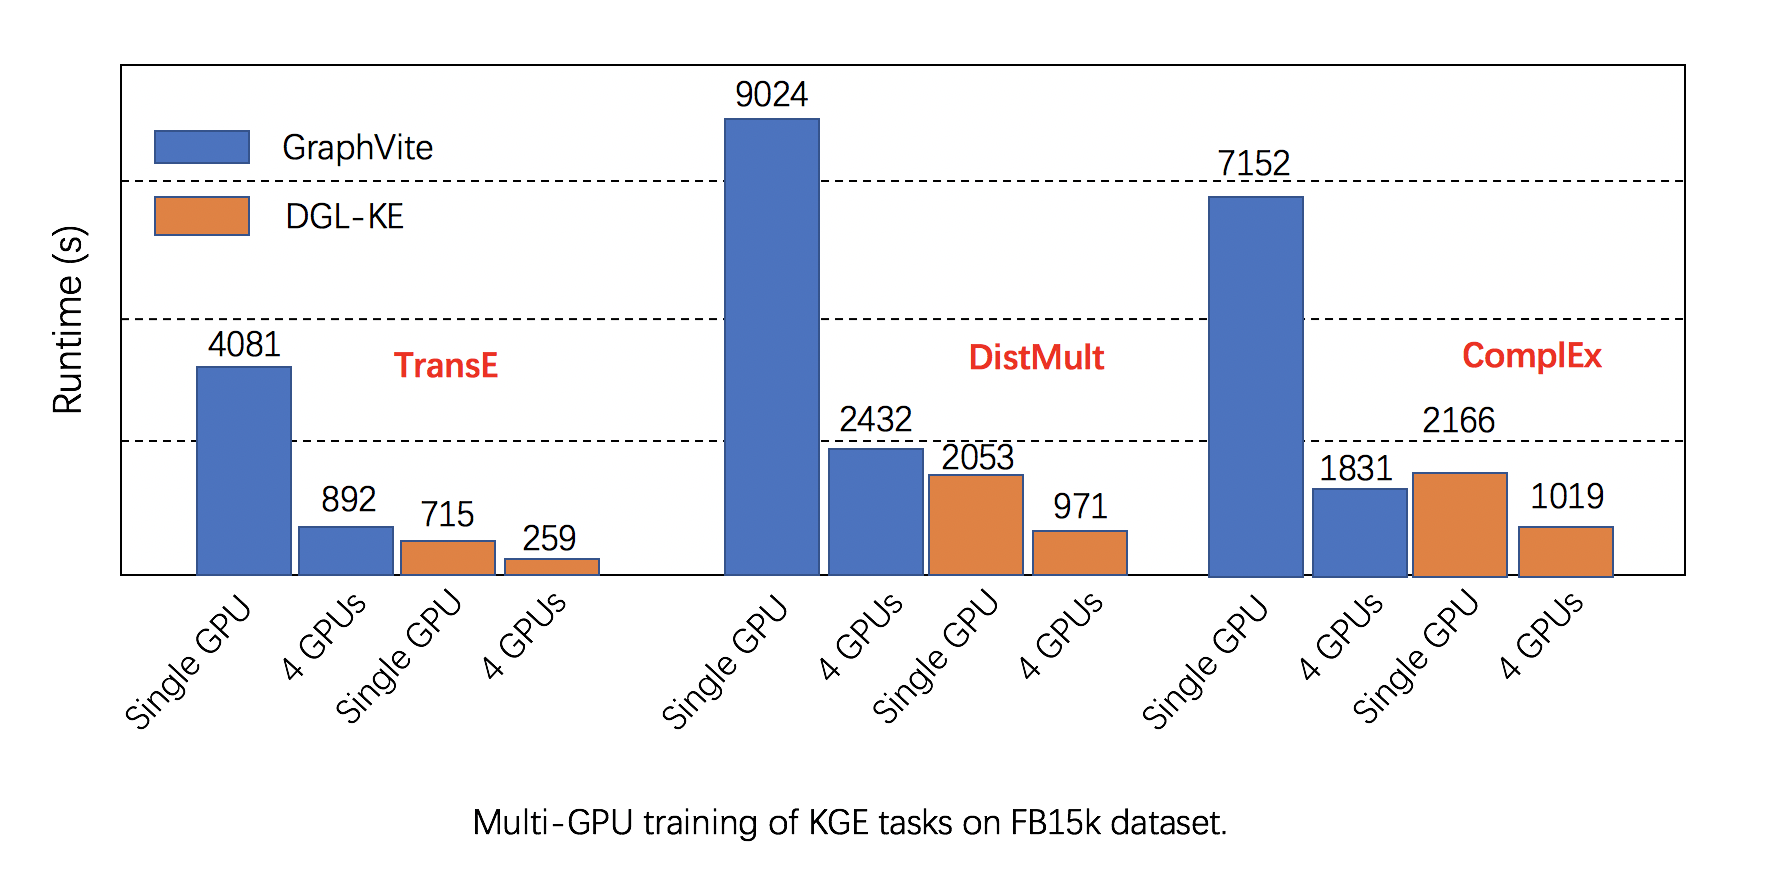
\includegraphics[width=0.9\linewidth]{images/one-four-GPUs-DGLvsGraphVite}
  \label{fig:sub2}
\end{subfigure}
\caption{Skalowalność DGL na wielu GPU oraz porównanie skalowalności na tle innej biblioteki}
\label{fig:test}
\end{figure}

\paragraph{}

DGL zapewnia szeroki zakres konwersji pomiędzy strukturami danych a grafami. Graf można wygenerować:
\begin{itemize}
    \item
    za pomocą: biblioteki NetworkX
    \item
    z tensora pochodzącego z biblioteki PyTorch
    \item
    z tablicy NumPy
    \item
    z macierzy adjacencji
    \item
    z listy krawędzi
\end{itemize}

Oprócz tego warto wspomnieć, że zarówno wierzchołkom jak i krawędziom można nadawać odpowiednie właściwości, a mianowicie w przypadku wierzchołkom mogą być to odpowiednie features używane do uczenia modelu, natomiast w przypadku krawędzi mogą to być tez wagi.

\paragraph{}
DGL jest uważana za łatwą w użyciu, wydajną i skalowalną biblioteką języka Python do głębokiego uczenia na strukturze grafu.
\paragraph{}
Główne cechy DGL:
\begin{itemize}
  \item
  integracja z wybranymi platformami do uczenia głębokiego - brak kosztów migracji, 
  \item 
  osiągnie wysokiej wydajności poprzez automatyczne grupowanie obliczeń i szybkie mnożenie macierzy rzadkich,
  \item 
  dobra skalowalność do wykresów z dziesiątkami milionów wierzchołków,
  \item 
  przejrzyste interfejsy dostępu do wierzchołków oraz krawędzi grafu, możliwość manipulacji strukturą grafu,
  \item 
  przekazywanie wiadomości (message passing) - zarówno niskopoziomowo np. przekazywanie informacji wzdłuż krawędzi i otrzymywanie ich na wybranych węzłach, jak i wysokopoziomowo np. aktualizowanie cech całego grafu.
  
 \end{itemize}

\section{Struktura biblioteki}
\label{sec:dgl_structure}
Źródła DGL \cite{dgl_sources} podzielone są na następujące moduły:
\begin{itemize}
  \item backend - odpowiedzialny za przygotowanie wspólnego API dla wywołań metod frameworków, które mogą być użyte jako baza dla działania DGL \cite{dgl}, takich jak: PyTorch \cite{torch}, Tensorflow \cite{tf}, MXNet \cite{mxnet}, czy numpy \cite{np}. Jest to klasyczne rozwiązanie dla bibliotek będąch wysokopoziomowymi wrapperami na grupę bibliotek niższego poziomu stanowiących implementację zbioru wspólnych operacji dla rowziązywania pewnego problemu. Podobną architekturę zobaczyć można w przypakdu biblioteki Keras \cite{keras}. Z poziomu biblioteki DGL \cite{dgl} wysokopoziomowe operacje wykonywane są za pomocą wspólnego API dla wszystkich obsługiwanych bibliotek bazowych.   
  \item contrib - w którym znajdują się rozszerzenia przygotowane przez społeczność.
  \item data - gdzie umieszczone są obiekty pośredniczące w dostępie do popularnych źródeł danych - ułatwia to szybkie rozpoczęcie eksperymentów, gdyż takie rowziązanie pozwala na pominięcie w dużej części przypadków narzutu czasowego na przygotowanie wygodnej warstwy dostępu do danych i konwersji na odpowiedni format, który jest akceptowany przez bibliotekę.
  \item function - w którym umieszczono kod odpowiedzialny za podstawe działania mechanizmu funkcji (w tym udf - user defined functions) operujących na elementach grafu.
  \item model\_zoo - zawierający zestaw predefiniowanych modeli sieci neuronowych opertych na publikacjach naukowych.
  \item nn - który zawiera implementacje najważniejszych dla grafowych sieci neuronowych operacji (dla wspieranych frameworków bazowych).
  \item runtime - gdzie umieszczono oniekty sterujące wykonaniem m. in. funkcji na elementach grafu.
  \item sampling - zawierający kod pozwalający na próbkowanie elementów grafu.
\end{itemize}
  
 \paragraph{}

 Od strony strukturalnej biblioteka prezentuje bardzo wysoki poziom przejrzystości, który świadczy o dobrej organizacji źródeł. Niestety przyznać należy, że nie wszystko zostało przygotowane w sposób ułatwiający korzystanie. Podczas instalacji pakietu z pip zauważyć można, że zależności do bibliotek bazowych nie zostają zainstalowane. Wymaga to wiedzy odnośnie wersji tych bibliotek, które są wymagane do poprawnej pracy DGL \cite{dgl}. Co więcej podczas testów wystąpiły problemy ze współpracą ze współdzielonymi bibliotekami CUDA \cite{cuda}, który udało się rozwiązać przez zainstalowanie (w teorii) nieodpowiedniej wersji pakietu DGL \cite{dgl}.

 \paragraph{}
 Na poziomie struktury interfejs głównych obiektów udostępnianych przez DGL \cite{dgl} jest stosunkowo prosty i czytelny. Biblioteka udostępnia klasy reprezentujący graf (DGLGraph będąca klasą bazową oraz DGLHeteroGraph dla grafów z typowanymi wierzchołkami pozwalająca na uzyskanie podobnego gfrafu wiedzy jak w grafowych bazach danych). Za pomocą interfejsu tych klas dokonać można szeregu operacji włącznie z transformacjami, próbkowaniem i konwersja grafu do i z różnych formatów. Na pochwałę zasługuje wprowadzenie kownersji na i z obiektów biblioteki NetworkX \cite{nx}.  Na ogół udostępnione metody są zaprojektowane w sposób bardzo przemyślany. Niestety nie ma to zastosowania w każdym przypadku. Przykładem może być brak możliwości stworzenia obiektu grafu wprost z gęstej macierzy sąsiedztwa, czy konieczność stworzenia pustego obiektu celem użycia metody konwersji z macierzy rzadkiej. Rzeczą wprost niezrozumiałą jest jednak błąd który pojawia się w konwersji z i rzadką macierz sąsiedztwa. W tym wypadku odtworzenie grafu z jego własnej macierzy sąsiedztwa powoduje zamianę kierunku krawędzi na przeciwny.

\paragraph{}
Biblioteka DGL \cite{dgl} prezentuje się zatem jako twór dość dobrze przemyślany, jednak wciąż posiadający sporo istotnych mankamentów utrudniających podstawowe wykorzystanie. Jednocześnie widać dość duże zainteresowanie społeczności i intensywny rozwój, co bardzo dobrze rokuje na przyszłość.

\section{Wymagania techniczne}
\label{sec:dgl_system_requirements}
\begin{itemize}
\item
DGL w wersji \textbf{0.4.x} współpracuje z następującymi systemami operacyjnymi:
\begin{itemize}
  \item
    Ubuntu 16.04    
  \item
    macOS X
  \item
   Windows 10
 \end{itemize}
\item
Rekomendowana wersja języka to Python 3.5 lub nowszy (biblioteka nie była testowana dla wersji niższych i może nie być z nimi kompatybilna). 
\item
Zalecana instalacja przy użyciu systemu zarządzania pakietami \textit{pip} lub \textit{conda}. Istnieje także możliwość instalacji poprzez pobranie plików źródłowych z GitHub \cite{dgl_sources}.
 \end{itemize}


\section{Opis eksperymentów}
\label{sec:experiments}
\paragraph{}
Jako podstawa dla niniejszego raportu został wykonanany szereg eksperymentów prezentujących praktyczną użyteczność biblioteki DGL \cite{dgl} przy rozwiązywaniu problemów z zakresu przetwarzania grafów.

\subsection{Częściowo nadzorowana klasyfikacja wierzchołków}
\paragraph{}
W ramach eksperymentu, na podstawie prostej symulacji rozprzestrzeniania się wirusa zostało sprawdzone w jaki sposób użyć biblioteki DGL \cite{dgl} do klasyfikacji wierzchołków przy użyciu podejscia zaprezentowanego w \cite{gcn} w warunkach posiadania jedynie niewielkiej ilosci etykiet. Rozwiązanie należy uznać z przydatne i dość istotne - zwłaszcza w obliczu globalnej pandemii. System badający kontakty międzyludzkie (na przykład na podstawie danych z urządzeń mobilnych), który potrafiłby określić potencjalnych chorych na bazie przeprowadzonych testów byłby bardzo cenny w wyżej wymienionych okolicznościach.

\paragraph{}
Symulacja obejmowała umieszczenie osobników w przestrzeni 2D i udostępnienie im możliwości ruchu w dowolnym kierunku o ograniczoną w ramach jednego kroku symulacji odległość. Osobniki będące w danym kroku symulacji w tym samym punkcie przestrzeni mogą wchodzić ze sobą w interakcje, kóre powodują ich wzajemną ekspozycję w skali $e_{o_1, o_2, x, y, t} \in [0.0; 1.0]$. Dla każdej pary osobników w danym punkcie przestrzeni i w danym punkcie czasu symulacji ($k_{o_1, o_2, x, y, t}$) zostaje wylosowana wartość $e_{o_1, o_2, x, y, t}$. Wirus, którego rozprzestrzenianie się odzwierciedla symulacja cechuje się współczynnikiem przenośności $a \in [0.0; 1.0]$ obrazującym jego zaraźliwość. Prawdopodobieństwo transmisji wirusa $P(k_{x, y, t})$ obliczne jest ze wzoru $P(k_{o_1, o_2, x, y, t}) = e_{o_1, o_2, x, y, t} * a$.

\paragraph{}
Z technicznego punktu widzenia wykonanie eksperymentu było stosunkwo proste, jako że biblioteka udostępnia dość wysoki poziom abstrakcji nad dość skomplikowanymi operacjami matematycznymi wykonywanymi w ramach trenowania grafowych sieci konwolucyjnych \cite{gcn}. Zgodnie z propozycją zawartą w \cite{gcn} wykorzystano ciągłą (co do wartości) macierz sąsiedztwa dla reprezentowania grafu celem odzwierciedlenia wartości $e_{o_1, o_2, x, y, t}$ już na poziomie struktury grafu, tak aby sieć neuronowa była uczona w kontekście głęboko osadzonym w strukturze projektu. Uproszczone rozwiązanie nie zakładało jednak wstrzykiwania do modelu sieci neuronowej informacji o ewolucji grafu w czasie, gdyż wymagałoby to sporej ilości pracy czysto koncepcyjnej nad architekturą modelu sieci neuronowej, która była poza zakresem działań w ramach projektu. Z racji przyjęcia zaprezentowanego sposobu przedstawienia problemu najbardziej właściwa metoda reprezentacji grafu to macierz sąsiedztwa (w przypadku dużych grafów w wersji rzadkiej), a w dalszej kolejności lista krawędzi (wraz z ich wagami) pozwalająca w sposób stosunkowo łatwy (jednak wymagający kosztu $O(E)$) wygenerować rzadką macierz sąsiedztwa. Lista wierzchołków może również być przekształcona w macierz sąsiedztwa dodatkowym kosztem $O(E)$ dla uzyskania macierzy rzadkiej. Etykiety węzłów wygodnie jest przechowywać w liście opisującej cechy każdego z nich, niezależnie od reprezentacji (informacja ta może być dołączana naturalnie w przypadku listy wierzchołków).

\paragraph{}
Wspomniany już wysoki poziom abstrakcji biblioteki DGL \cite{dgl} umożliwił sprawne wykonanie eksperymentu i jest cechą, którą należy rozpatrywać pozytywnie. Należy jednak pamiętać, że zbyt duży poziom abstrakcji w ogólnym przypadku powodować może utratę kontroli nad przebiegiem eksperymentu i przynieść skutki odwrotne do zamierzonych. Pod tym względem obawiać się można problemów analogicznych do tych, które występowały w bibliotece Keras \cite{keras} na początkowych etapach jej rowzoju (jak i wówczas kiedy była już oficjalnie częscią TensorFlow \cite{tf}). Problemy te objawiały się m. in. pojawiającymi się zakleszczeniami, czy wyciekami pamięci. Zauważyć jednak należy, że w przypadku DGL \cite{dgl} z wykorzystaniem biblioteki PyTorch \cite{torch} możliwa jest manualna kontrola procesu uczenia, która może niwelować szanse wystąpienia w/w problemów. Pomimo przedstawionych obaw. w ogólności działanie DGL \cite{dgl} w czasie eksperymentu ocenić należy bardzo dobrze.


\subsection{Wykrywanie wspólnot (Community Detection)}
\paragraph{}
Wykrywanie wspólnot w sieci połączeń polega na odnajdywaniu podgrup odznaczających się wspólnymi cechami. Wspólnoty obejmują podgrafy sieci z wysoką liczbą połączeń pomiędzy wierzchołkami tego samego podgrafu i relatywnie mniejszą liczbą połączeń z wierzchołkami innych podgrafów. Struktura sieci nie wykazuje jednorodności, a raczej cechuje ją podział na klasy z wyższym prawdopodobieństwem połączeń między węzłami tej samej klasy niż między węzłami różnych klas \cite{community_detection}. Dla danej sieci reprezentowanej przez graf \(G = (V, E)\) , gdzie \(V\) jest zbiorem wierzchołków, a \(E\) zbiorem krawędzi, struktura wspólnoty to taki podział wierzchołków \(V\) na zbiory \(C = C_{1},..., C_{k}\) tak, że każdy \(C_{i}, 1 \leq i \leq	 k\) wykazuje strukturę wspólnoty reprezentujące grupy węzłów.

\paragraph{}
Do przykładów takich sieci można zaliczyć m.in. sieci społecznościowe, gdzie połączenia pokazują powiązania między osobami, systemy rekomendujące, w których połączenia pokazują interakcje między klientami a produktami i procesy analizy chemicznej, w której związki są modelowane jako połączenia atomów i wiązań \cite{network_community_detection}. Zrozumienie struktury sieci połączeń i wykrywanie wspólnot ma kluczowe znaczenie dla wydobycia przydatnych informacji. Dzięki poznaniu zależności pomiędzy poszczególnymi komponentami można wykorzystać posiadaną wiedzę np. w marketingu docelowym czy naukach o naturze. 

\paragraph{}
Biorąc pod uwagę, że interakcje między klientami a produktami są dobrym przykładem sieci umożliwiających wykrywanie wspólnot eksperyment został przeprowadzony na zbiorze danych Polbooks \cite{polbooks}. Zbiór ten reprezentuje sklasyfikowany zestaw książek o tematyce polityki USA. Został on stworzony na podstwie danych z serwisu Amazon.com zgodnie z powiązaniem: „klienci, którzy kupili tę książkę, również kupili te książki”. Składa się on z 105 książek i 441 powiązań pomiędzy nimi. 

\paragraph{}
Zadaniem eksperymentu było sprawdzenie czy biblioteka DGL, przy użyciu grafowych sieci konwolucyjnych i uczenia częściowo nadzorowanego, nadaje się do wykrywania wspólnot w danych o strukturze grafowej. Aby to zweryfikować stworzono dwa rozwiązania: pierwsze z małym podzbiorem zbioru Polbooks (12 książek i 25 połączeń między nimi, zachowując proporcje odpowiednich kategorii) oraz drugie z całością danych. Pierwszym krokiem było ustalenie jakie parametry GCN będą odpowiednie dla pierwszego rozwiązania, żeby zastosować je w większej skali (ze względu na to, że łatwiej obserwować trenowanie danych na mniejszej ich ilości). Drugim było zastosowanie wytworzonego modelu dla całości danych.


\paragraph{}
Niestety można mieć mieszane odczucia jeśli chodzi o korzystanie z tej biblioteki w celu wykonania tego zadania.
Z jednej strony nie było problemów z integracją biblioteki PyTorch, konwersją grafu do i z obiektu biblioteki NetworkX oraz obsługą danych grafowych. Z drugiej jednak napotkano dość duże problemy z dobraniem prawidłowych parametrów modelu sieci, szczególnie dotyczących liczby wartw ukrytych oraz ich rozmiarów. Resumując, wydaje się że DGL to dobra biblioteka do realizacji zadania jakim jest wykrywanie wspólnot lecz metody jakie są przez nią udostępniane zmuszają do spędzenia dużej ilości czasu na dostrajaniu parametrów sieci, co nadaje to zastosowanie bardziej badawczo-naukowe niż gotowe do użycia w produkcji.

\subsection{Wykorzystanie Heterografów w uczeniu maszynowym}
\paragraph{}
Według publikacji 'A Survey of Heterogeneous Information Network Analysis' \cite{heteropaper} ważnym elementem dzisiejszych systemów informatycznych jest fakt, że składają się z wielu komponentów stale komunikujących się między sobą, a większość współczesnych naukowców modeluje je za pomocą sieci homogenicznych. Tego typu sieci nie pozwalają na rozróżnianie różnych typów obiektów (wierzchołków w grafie) czy też różnych rodzajów połączeń (krawędzi w grafie) w sieciach. Dlatego też coraz więcej badaczy rozpatruje bardziej skomplikowane połączenia jako sieci heterogeniczne. Sieci informacyjne zbudowane z heterografów mogą zawierać bogatszą strukturę oraz informacje semantyczne, które zapewniają wiele możliwości rozwoju analizy specyficznego rodzaju danych.

\paragraph{}
Biblioteka DGL wspiera obliczenia na grafowych sieciach neuronowych z użyciem klasy heterogenicznych grafów wraz z odpowiednim API. W jej ramach możemy tworzyć heterografy między innymi z połączenia kilku grafów, grafów dwudzielnych czy też listy relacji. Możliwa jest również konwersja w drugą strone na sieć NetworkX lub na homograf. Ciekawymi przykładami grafów heterogenicznych, które zostały poruszone w ramach dokumentacji DGL \cite{dgl} niech będą:

\begin{itemize}
  \item Citation graph (graf cytowań) - Opierając się na datasecie stworzonym przez The Association for Computing Machinery, który zawiera informację o publikacjach, ich autorów, miejsca, gdzie publikacje się ukazały, a także co ważne publikacje, które cytują inne. Wszystkie te informację mogą zostać zapisane i zwizualizowane za pomocą grafów heterogenicznych. Przykładowo możemy wyróżnić następujące relacje: (P) publikacja napisana przez (A) autora, (P) publikacja opublikowana na łamach danego (V) czasopisma, oraz (P) publikacja cytującą inne.
  
  \item Recommender systems (system rekomendacji) - innym przykładem ciekawym z punktu widzenia chociażby grafowych baz danych może być system rekomendacji, gdzie występują interakcję pomiędzy użytkownikami i pewnymi elementami systemu. Jako przykładem posłużmy się ratingami filmów ocenianymi przez użytkowników. Tego typu interakcje można reprezentować za pomocą heterografów - wierzchołki dwóch typów (użytkownicy i filmy) oraz krawędzie dwóch rodzajów (ocena pozytywna lub negatywna). 
  
  \item Knowledge graph (graf wiedzy) - do reprezentowania relacji pomiędzy poszczególnymi osobami oraz ich rolami,  a także elementów które je ze sobą łączą. 

\end{itemize}

\paragraph{}
Jak już zostało wspomniane powyżej, DGL pozwala na uczenie maszynowe z użyciem grafów heterogenicznych. W naszym eksperymencie posłużyliśmy się grafem cytowań stworzonym na podstawie datasetu The Association for Computing Machinery, który zawiera ponad 2 mln różnych publikacji. Celem eksperymentu było przewidzenie z którą konferencją jest związana dana publikacja. Aby zachować charakter uczenia maszynowego częściowo nadzorowanego wybraliśmy tylko kilka spośród konferencji, aby zostały olabelowane. Do nauki modelu posłużyliśmy się relacyjnym GCN o następującym wzorze przekazywania wiadomości: $ h_{i}^{l+1} = \sigma (\sum_{r \epsilon R}\sum_{j \epsilon N_{r}(i))} W
_{r}^{l}h_{j}^{l}) $. Sieć heterogeniczna wykorzystana w tym przykładzie, trzyma w sobie wagi poszczególnych relacji, następnie specyfikujemy funkcję forward, która zawiera funkcję odpowiedzialną za agregację wag relacji oraz za ich poprawną redukcję. Tak wytrenowany model, poddajemy ewaluacji, która zwraca obiecujące rezultaty zachowując odpowiednią wydajność obliczeń. 

\paragraph{}
Innym aspektem związanym z heterografami jest link prediction, czyli predykcja czy pomiędzy parą wierzchołków istnieje krawędź danego typu lub znalezienie które wierzchołki są połączone z wierzchołkiem danego typu. Eksperymentowaliśmy na zbiorze treningowym FB15K zawierającym tysiące wierzchołków i relacji pomiędzy nimi. Była to równocześnie próba przeprowadzenia obliczeń na GPU, która w bardzo dużym stopniu zoptymalizowała szybkość wykonywanych obliczeń. W rezultacie testu na dosyć ograniczonym ze względu na zasoby obliczeniowe zbiorze otrzymaliśmy rezultat na poziomie 80\% skuteczności.  

\section{Wnioski}
\label{sec:conclusions}
Reasumując jak pokazała analiza przeprowadzona w ramach tego dokumentu, biblioteka DGL jest stale rozwijającym się rozwiązaniem służącym do reprezentowania grafowych struktur danych. Mimo pewnych niedoskonałości wynikającym z niedopracowania w pełni niektórych elementów tej biblioteki, możemy ją uznać za dosyć dobry wybór do wykonania pewnych eksperymentów analizy danych. Co warto dodać wypada także lepiej na tle konkurencyjnych rozwiązań w kwestii wydajności i skalowalności. Coraz bardziej rosnące zainteresowanie społeczności naukowej tematyką przetwarzania grafów z użyciem uczenia maszynowego, może przynieść bibiotece dalszy rozwój oraz dopracowanie niektórych jej mankamentów. 

\bibliographystyle{unsrt}  
%\bibliography{references}  %%% Remove comment to use the external .bib file (using bibtex).
%%% and comment out the ``thebibliography'' section.


%%% Comment out this section when you \bibliography{references} is enabled.
\clearpage
\renewcommand\refname{Źródła}
\begin{thebibliography}{1}

\bibitem{dgl} 
\newblock Deep Graph Library. 
\newblock {\em https://www.dgl.ai/}

\bibitem{dgl_sources} 
\newblock Źródła Deep Graph Library. 
\newblock {\em https://github.com/dmlc/dgl/tree/0.4.x}

\bibitem{torch} 
\newblock PyTorch. 
\newblock {\em https://pytorch.org/}

\bibitem{tf} 
\newblock TensorFlow. 
\newblock {\em https://www.tensorflow.org/}

\bibitem{mxnet} 
\newblock MXNet. 
\newblock {\em https://mxnet.apache.org/}

\bibitem{np} 
\newblock numpy. 
\newblock {\em https://numpy.org/}

\bibitem{keras} 
\newblock Keras. 
\newblock {\em https://keras.io/}

\bibitem{cuda} 
\newblock CUDA. 
\newblock {\em https://developer.nvidia.com/cuda-zone}

\bibitem{nx} 
\newblock NetworkX. 
\newblock {\em https://networkx.github.io/}

\bibitem{gcn} 
Kipf T., Welling M.:
\newblock Semi-Supervised Classification with Graph Convolutional Networks,
\newblock {\em arxiv:1609.02907}, 2016

\bibitem{community_detection} 
Hric D., Darst R. K., Fortunato S.:
\newblock Community detection in networks: Structural communities versus ground truth,
\newblock {\em arXiv:1406.0146}, 2014

\bibitem{network_community_detection} 
Khan B. S., Niazi M. A.:
\newblock Network Community Detection: A Review and Visual Survey,
\newblock {\em arXiv:1708.00977}, 2017

\bibitem{polbooks} 
\newblock Polbooks dataset. 
\newblock {\em http://www-personal.umich.edu/~mejn/netdata/polbooks.zip}

\bibitem{heteropaper} 
\newblock Heteregenous Graph. 
\newblock {\em https://arxiv.org/pdf/1511.04854.pdf}

\end{thebibliography}



\end{document}